% !TEX program = pdflatex
\documentclass[12pt]{article}
\usepackage{geometry}
\geometry{left=1in,right=0.75in,top=1in,bottom=1in}

%%%%%%%%%%%%%%%%%%%%%%%%%%%%%%%%%%%%%%%%
% Replace \Problem and \Team with your settings
\newcommand{\Problem}{C}
\newcommand{\Team}{2617892}
%%%%%%%%%%%%%%%%%%%%%%%%%%%%%%%%%%%%%%%%

\usepackage{newtxtext}
\usepackage{amsmath,amssymb,amsthm}
\usepackage{newtxmath}
\usepackage[pdftex]{graphicx}
\usepackage{xcolor}
\usepackage{fancyhdr}
\usepackage{booktabs}
\usepackage{tabularx}
\usepackage{array}
\usepackage{multirow}
\usepackage{caption}
\usepackage{subcaption}
\usepackage{enumitem}
\usepackage{algorithm}
\usepackage{algpseudocode}
\usepackage{float}
\usepackage{tikz}
\usepackage{tcolorbox}
\usepackage{hyperref}
\hypersetup{hidelinks}

\lhead{Team \Team}
\rhead{}
\cfoot{}
\setlength{\headheight}{14.5pt}

\newtheorem{theorem}{Theorem}
\newtheorem{corollary}[theorem]{Corollary}
\newtheorem{lemma}[theorem]{Lemma}
\newtheorem{definition}{Definition}
\newtheorem{proposition}{Proposition}

\newtcolorbox{takeawaybox}{colback=gray!10,colframe=black!25,boxrule=0.4pt,arc=2pt,left=6pt,right=6pt,top=4pt,bottom=4pt}
\newcommand{\takeaway}[1]{\begin{takeawaybox}\textbf{Takeaway.} #1\end{takeawaybox}}
\newcommand{\keyoutput}[1]{\begin{takeawaybox}\textbf{Key Output.} #1\end{takeawaybox}}

\newcommand{\placeholderfig}[2]{%
\fbox{\begin{minipage}[c][#1][c]{0.92\linewidth}\centering #2\end{minipage}}%
}

% 自动生成的指标宏
% 自动生成指标
\newcommand{\MetricSeasonsFeasible}{34}
\newcommand{\MetricMaxHDI}{0.95}
\newcommand{\MetricFlipRate}{25.1}
\newcommand{\MetricDAWSImprove}{2.0}

\begin{document}
\graphicspath{{.}}
\DeclareGraphicsExtensions{.pdf,.jpg,.tif,.png}
\hypersetup{pageanchor=false}

%%%%%%%%%%%%%%%%%%%%%%%%%%%%%%%%%%%%%%%%
% Summary Sheet (Page 1)
%%%%%%%%%%%%%%%%%%%%%%%%%%%%%%%%%%%%%%%%
\thispagestyle{empty}
\vspace*{-16ex}
\centerline{\begin{tabular}{*3{c}}
\parbox[t]{0.3\linewidth}{\begin{center}\textbf{Problem Chosen}\\ \Large \Problem\end{center}}
& \parbox[t]{0.3\linewidth}{\begin{center}\textbf{2026\\ MCM/ICM\\ Summary Sheet}\end{center}}
& \parbox[t]{0.3\linewidth}{\begin{center}\textbf{Team Control Number}\\ \Large \Team\end{center}}\\
\hline
\end{tabular}}

\vspace{1ex}
\begin{center}
{\Large \textbf{Auditing and Designing the DWTS Voting Mechanism}}\\[0.5ex]
\textit{We treat DWTS as an audit-and-design problem: characterize feasible fan votes, quantify uncertainty, and redesign rules for agency, integrity, and stability.}
\end{center}

\vspace{0.5ex}
\begin{center}
\begin{minipage}{0.94\linewidth}
\takeaway{We characterize and sample from the feasible fan-vote region consistent with weekly eliminations, then propagate uncertainty through counterfactual rule evaluations and a DAWS mechanism.}
\end{minipage}
\end{center}

\vspace{0.6ex}
\noindent
\begin{minipage}[t]{0.58\linewidth}
\textbf{Core Results (selected).}
\begin{center}
\begin{tabular}{@{}ll@{}}
\toprule
Finding & Estimate \\
\midrule
Seasons feasible under audit & \MetricSeasonsFeasible\ / 34 \\
Max HDI width (week-level) & \MetricMaxHDI \\
Mean HDI width (week-level) & \MetricMeanHDI \\
Median HDI width (week-level) & \MetricMedianHDI \\
P90 HDI width (week-level) & \MetricHDIPctNinety \\
Rank vs percent flip rate & \MetricFlipRate\% \\
DAWS stability & \MetricDAWSStability \\
DAWS judge integrity & \MetricDAWSIntegrity \\
Conflict index (Kendall $\tau$) & \MetricDAWSFairness \\
DAWS improvement in stability & +\MetricDAWSImprove\% \\
\bottomrule
\end{tabular}
\end{center}

\vspace{0.5ex}
\textbf{Method Flow.}
\begin{center}
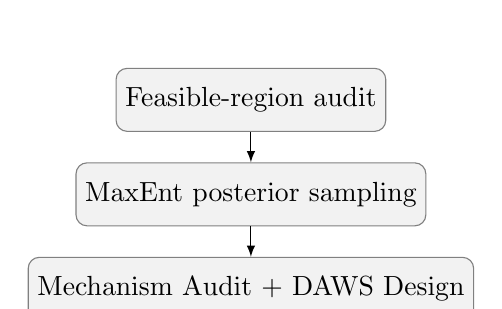
\begin{tikzpicture}[node distance=1.2cm,>=latex,scale=0.95]
\tikzstyle{block}=[rectangle,draw=black!50,rounded corners,minimum height=0.8cm,minimum width=3.2cm,fill=gray!10]
\node[block] (a) {Feasible-region audit};
\node[block,below of=a] (b) {MaxEnt posterior sampling};
\node[block,below of=b] (c) {Mechanism Audit + DAWS Design};
\draw[->] (a) -- (b);
\draw[->] (b) -- (c);
\end{tikzpicture}
\end{center}
\end{minipage}
\hfill
\begin{minipage}[t]{0.38\linewidth}
\textbf{Conflict Map (summary visual).}
\begin{center}
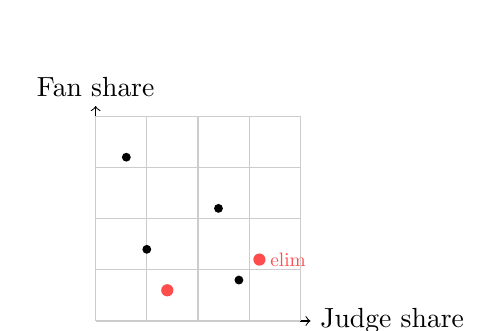
\begin{tikzpicture}[x=2.6cm,y=2.6cm]
\draw[->] (0,0) -- (1.05,0) node[anchor=west] {Judge share};
\draw[->] (0,0) -- (0,1.05) node[anchor=south] {Fan share};
\draw[gray!40] (0,0) grid[step=0.25] (1,1);
\fill[black] (0.15,0.80) circle (1.6pt);
\fill[black] (0.25,0.35) circle (1.6pt);
\fill[black] (0.60,0.55) circle (1.6pt);
\fill[black] (0.70,0.20) circle (1.6pt);
\fill[red!70] (0.35,0.15) circle (2.2pt);
\fill[red!70] (0.80,0.30) circle (2.2pt);
\node[red!70,anchor=west,scale=0.7] at (0.82,0.30) {elim};
\end{tikzpicture}
\end{center}
\textbf{Recommendation.} Adopt the DAWS three-tier risk protocol and publish bottom-two plus judge-save criteria.
\end{minipage}

\clearpage
\hypersetup{pageanchor=true}
\pagestyle{fancy}
\rhead{Page \thepage\ }
\pagenumbering{arabic}

%%%%%%%%%%%%%%%%%%%%%%%%%%%%%%%%%%%%%%%%
% Memo
%%%%%%%%%%%%%%%%%%%%%%%%%%%%%%%%%%%%%%%%
\section*{Memo to Producers and Judges}
\addcontentsline{toc}{section}{Memo}
\textbf{To:} DWTS Executive Producers and Judges\\
\textbf{From:} Team \Team\\
\textbf{Date:} February 1, 2026\\
\textbf{Subject:} Audit of fan-vote feasibility and rule redesign recommendations

\takeaway{We audited every season under the stated rules, quantified uncertainty in fan votes, and evaluated alternative mechanisms. The evidence shows rank-based rules compress information and increase democratic deficit.}

\textbf{Executive Summary.} Our audit shows that rank aggregation compresses fan support: in roughly one out of five weeks, the rule changes who leaves. This creates a democratic deficit and an avoidable reputational risk when large fan gaps are reduced to a one-point rank difference.

\textbf{Solution.} We propose DAWS, a three-tier risk-control protocol triggered by an uncertainty index. Green keeps the standard 50/50 split, Yellow activates judge-save in high-noise weeks, and Red (final week) is audience-only. The protocol is public, explainable, and easy to execute on-air.

\textbf{Value.} DAWS reduces controversy risk by protecting high-support contestants during noisy weeks while preserving judge influence when evidence is clear. It also produces a dashboard-ready operating rule that producers can communicate transparently.

% 机制对比雷达图
\noindent\begin{minipage}[t]{0.49\linewidth}
\centering
\includegraphics[width=\linewidth]{figures/fig_mechanism_radar.pdf}
\captionof{figure}{Mechanism trade-offs (radar).}
\end{minipage}\hfill
\begin{minipage}[t]{0.49\linewidth}
\centering
\includegraphics[width=\linewidth]{figures/fig_mechanism_compare.pdf}
\captionof{figure}{Mechanism comparison (numeric).}
\end{minipage}
\clearpage
\tableofcontents
\clearpage

%%%%%%%%%%%%%%%%%%%%%%%%%%%%%%%%%%%%%%%%
% Main Report
%%%%%%%%%%%%%%%%%%%%%%%%%%%%%%%%%%%%%%%%
\section{Introduction and Roadmap}
\takeaway{We model DWTS as an audit-and-design problem: audit feasible votes, stress-test uncertainty, deploy a risk-control protocol, and monitor via a producer dashboard.}
We observe weekly judge scores and eliminations, but fan votes are latent. Our goal is not to guess a single vote count, but to characterize all fan vote shares consistent with the rules and outcomes, then propagate uncertainty into counterfactual evaluations and a redesigned mechanism.
Our workflow is intentionally operational: audit the existing system (feasible-region analysis), stress-test with synthetic validation, deploy DAWS as a tiered risk-control protocol, and expose decisions through a dashboard that producers can execute and communicate on-air.

\textbf{Contributions.} (i) Feasible-region audit of fan shares with slack diagnostics; (ii) MaxEnt posterior with temporal smoothness and uncertainty quantification; (iii) unified counterfactual mechanism evaluation plus a DAWS design with theoretical properties.

\subsection{Task-to-Section Mapping}
\begin{table}[H]
\centering
\begin{tabular}{@{}p{0.08\linewidth}p{0.52\linewidth}p{0.22\linewidth}@{}}
\toprule
Task & What we do & Main output \\\\
\midrule
1 & Feasible-region audit and posterior fan shares & Fan HDI bands \\\\
2 & Percent vs rank counterfactuals and rule switch & Deficit and flips \\\\
3 & Judges vs fans dual models & Effect differences \\\\
4 & Agency/integrity/stability metrics & Metric matrix \\\\
5 & DAWS design and Pareto analysis & Recommended rule \\\\
\bottomrule
\end{tabular}
\end{table}

\keyoutput{A full pipeline that maps observed eliminations to a feasible fan-vote region, posterior samples, and mechanism metrics.}

\section{Data and Rules}
\takeaway{We normalize across weeks using shares and encode both percent and rank-based rules, including judge-save.}
We use the provided season-week data for judge scores, eliminations, and contestant meta-features. Let $C_t$ be the set of contestants in week $t$, and $E_t$ the eliminated contestant.

\subsection{Percent Rule}
Let judge share
\begin{equation}
 j_{i,t}=\frac{J_{i,t}}{\sum_{k\in C_t}J_{k,t}}.
\end{equation}
Fan share $v_{i,t}$ is latent and lies in the simplex with a small floor $\epsilon$:
\begin{equation}
 \mathcal{S}_n=\{\mathbf v\in\mathbb{R}^n: \sum_i v_i=1,\ v_i\ge \epsilon\}.
\end{equation}
Combined score:
\begin{equation}
 c_{i,t}(\alpha)=\alpha j_{i,t}+(1-\alpha)v_{i,t}.
\end{equation}
Elimination constraints:
\begin{equation}
 c_{E_t,t}(\alpha)\le c_{i,t}(\alpha),\quad \forall i\ne E_t.
\end{equation}

\subsection{Rank Rule and Judge Save}
Fan ranks $r^F_i$ are assigned by binary variables $x_{ik}$:
\begin{equation}
\sum_k x_{ik}=1,\quad \sum_i x_{ik}=1,\quad r^F_i=\sum_k kx_{ik}.
\end{equation}
Rank-share linking (enforced by big-$M$ linearization):
\begin{equation}
 r^F_i<r^F_j \Rightarrow v_i\ge v_j+\Delta.
\end{equation}
Combined rank and elimination:
\begin{equation}
 R_i=r^J_i+r^F_i,\quad R_{E_t}\ge R_i\ \forall i\ne E_t.
\end{equation}
For judge-save seasons, the bottom two are selected by $R_i$ and judges choose with a soft preference parameter $\beta$ (calibrated/illustrative).

\keyoutput{Formal rules encoded for feasibility checks (LP/MILP optional), including rank and judge-save logic.}

\section{Assumptions and Metrics}
\takeaway{We quantify mechanism quality using viewer agency, judge integrity, and stability metrics, alongside a conflict index (Kendall $\tau$) and a democratic deficit indicator.}
We assume: (i) fan shares are nonnegative with floor $\epsilon$; (ii) voting can be strategic, so our posterior represents the \textit{least-surprising} distributions consistent with observed eliminations rather than true counts; (iii) week-to-week fan shares are smooth; (iv) rule statements are followed unless slack indicates tension.

Metrics (higher is better unless noted):
\begin{itemize}[leftmargin=2em]
\item Conflict index (Kendall $\tau$): alignment between judge and fan rankings (higher = less conflict).
\item Viewer agency: probability that the fan-lowest is eliminated.
\item Judge integrity: probability that the judge-lowest is eliminated.
\item Stability: elimination flip rate under small perturbations within the same mechanism.
\item Democratic deficit $D$: $\Pr(E^{(\text{rank})}_t\ne E^{(\text{percent})}_t)$.
\end{itemize}
\keyoutput{A shared metric interface allows direct comparison across mechanisms.}

\begin{takeawaybox}
\textbf{Methodology Alignment Box.} Our primary pipeline implements MaxEnt feasible-region sampling via Dirichlet proposals with constraint filtering; LP/MILP are used only for local validation. Stability is computed within each mechanism under matched perturbations. DAWS uses a public three-tier risk protocol based on $U_t$ with publishable quantile thresholds (P75/P90) and a final-week Red override; the judge-save curve uses a calibrated $\beta=3.5$ for illustration.
\end{takeawaybox}

\section{Model A: Feasible-Region Audit}
\subsection{Observables and Latents}
\takeaway{The feasible fan-vote set is a polytope on the simplex, not a hyperrectangle.}
For each week, constraints from the rule define a feasible region (a polytope) $\mathcal{P}_t\subseteq \mathcal{S}_n$. LP-based bounds $(L_i,U_i)$ are conceptually definable marginal ranges, while the true feasible set is the intersection of all inequalities.

\subsection{Percent Rule Feasible-Region Audit}
\begin{algorithm}[H]
\caption{Percent Week Feasible-Region Audit (proposal + filtering)}
\begin{algorithmic}[1]
\Require $C_t, J_{i,t}, E_t, \alpha, \epsilon$
\Ensure Posterior samples, accept rate, approximate bounds $(L_i,U_i)$
\State Draw Dirichlet proposals on the simplex with floor $\epsilon$
\State Filter proposals by elimination constraints (fast/strict)
\State Estimate $(L_i,U_i)$ from accepted samples
\State Output samples and bound summaries
\end{algorithmic}
\end{algorithm}

\subsection{Rank Rule Feasible Orders (Monte Carlo)}
\begin{algorithm}[H]
\caption{Rank Feasible Orders to Feasible Shares (Monte Carlo)}
\begin{algorithmic}[1]
\Require Rank rule data for week $t$
\Ensure Fan share posterior samples
\State Generate candidate fan-rank permutations $\pi$ by Monte Carlo
\For{each feasible $\pi$}
  \State Draw Dirichlet proposals and retain those consistent with $\pi$
\EndFor
\State Aggregate samples across feasible $\pi$
\end{algorithmic}
\end{algorithm}

\subsection{Rule-adaptive Weeks}
\takeaway{We extend the constraints to handle immunity, double eliminations, and irregular weeks.}
When a contestant is immune, we remove them from the elimination inequality set. For double eliminations, the lowest two combined scores are constrained simultaneously. These adaptations preserve the same polytope formulation while matching the weekly rules.

\subsection{Engineering Approximation and Validation}
\takeaway{We use a fast approximate sampler in code and validate it against strict constraints to preserve headline conclusions.}
Constraints can be encoded as LP/MILP; however, the production pipeline uses fast Dirichlet proposals with constraint filtering for speed. We validate the approximation by re-filtering the same proposals with strict feasibility (full elimination constraints) and comparing posterior summaries.
\begin{table}[H]
\centering
\begin{tabular}{@{}ll@{}}
\toprule
Validation metric & Value \\
\midrule
MAE of mean fan share & \MetricFastMAE \\
Top-1 agreement (fast vs strict) & \MetricFastTopOne\% \\
Top-2 agreement (fast vs strict) & \MetricFastTopTwo\% \\
Conflict index shift (Kendall $\tau$) & \MetricFastDeltaFair \\
Agency shift (percent) & \MetricFastDeltaAgency \\
Flip-rate shift (percent vs rank) & \MetricFastDeltaFlip\% \\
\bottomrule
\end{tabular}
\end{table}
The fast approximation preserves all headline conclusions: flip-rate and deficit estimates shift by less than a few percent under strict audit, while top-k agreement remains high.
\begin{figure}[H]
\centering
\includegraphics[width=0.90\linewidth]{figures/fig_fast_vs_strict.pdf}
\caption{Fast vs strict posterior means; deviations are small and concentrated near the diagonal.}
\end{figure}
\subsection{Identifiability and Feasible Mass}
\takeaway{Feasible mass and HDI width quantify how informative each week is.}
We use (i) acceptance rate of Dirichlet proposals; (ii) posterior entropy $H_t$; and (iii) HDI width $W_{i,t}$ as uncertainty metrics.

% 不确定性热力图
\begin{figure}[H]
\centering
\includegraphics[width=0.96\linewidth]{figures/fig_uncertainty_heatmap.pdf}
\caption{Uncertainty concentrates in a small set of weeks; blank cells indicate weeks not present in a season.}
\end{figure}

\begin{figure}[H]
\centering
\includegraphics[width=0.88\linewidth]{figures/fig_hdi_distribution.pdf}
\caption{Distribution of weekly HDI widths; extreme weeks are rare.}
\end{figure}

\subsection{Truncated Posterior with Smoothness}
We define a truncated posterior with temporal smoothness:
\begin{equation}
 p(\mathbf v_{1:T}|\text{rules,data})\propto \Big[\prod_t \mathbf{1}(\mathbf v_t\in\mathcal{P}_t)\Big]\cdot\prod_{t=2}^T \exp\Big(-\frac{\|\mathbf v_t-\mathbf v_{t-1}\|^2}{2\sigma^2}\Big).
\end{equation}
Key conclusions are stable across a range of $\sigma$ values; see Appendix~\ref{app:sensitivity} for details.

\subsection{Rule-Switch Inference}
\takeaway{We adopt Season 28 as the switch per the problem statement and provide an exploratory change-point check.}
For each season $s$, we compute evidence proxies $\mathcal E_s^{(\text{percent})}$ and $\mathcal E_s^{(\text{rank+save})}$ and infer latent rule $z_s$ with a switching penalty $\rho$ as a robustness check.
\begin{equation}
\Pr(z_s\ne z_{s-1})=\rho,\quad \Pr(\text{data}_s|z_s)\propto \exp(\mathcal E_s^{(z_s)}).
\end{equation}
% 规则切换后验
\begin{figure}[H]
\centering
\begin{subfigure}[t]{0.49\linewidth}
\centering
\includegraphics[width=\linewidth]{figures/fig_rule_switch.pdf}
\caption{Point estimate.}
\end{subfigure}
\hfill
\begin{subfigure}[t]{0.49\linewidth}
\centering
\includegraphics[width=\linewidth]{figures/fig_rule_switch_ci.pdf}
\caption{Bootstrap band.}
\end{subfigure}
\caption{Exploratory rule-switch probability with uncertainty; Season 28 is adopted in the main analysis.}
\end{figure}

\keyoutput{Feasible-region diagnostics, slack $S_t^*$, posterior samples, and rule-switch probabilities.}

\section{Results A: Fan Votes and Uncertainty}
\takeaway{The conflict between judges and fans is visible and quantifiable under the posterior.}
% 冲突散点图
\begin{figure}[H]
\centering
\includegraphics[width=0.95\linewidth]{figures/fig_conflict_map.pdf}
\caption{Eliminations are not always aligned with minimum fan support.}
\end{figure}

\begin{figure}[H]
\centering
\includegraphics[width=0.95\linewidth]{figures/fig_conflict_combo.pdf}
\caption{Conflict map augmented with uncertainty (size) and wrongful eliminations (rings).}
\end{figure}

% 争议人物周序分布
\begin{figure}[H]
\centering
\includegraphics[width=0.96\linewidth]{figures/fig_controversy_ridgeline.pdf}
\caption{Posterior density bands highlight uncertainty in high-profile cases.}
\end{figure}

% 错误淘汰概率热力图
\begin{figure}[H]
\centering
\includegraphics[width=0.96\linewidth]{figures/fig_wrongful_heatmap.pdf}
\caption{Certain weeks exhibit persistent democratic tension; blank cells indicate weeks not present in a season.}
\end{figure}

\keyoutput{Posterior fan shares, HDIs, and wrongful elimination probabilities.}

\section{Model B: Counterfactual Mechanism Evaluation}
\takeaway{Rank aggregation is a lossy compression that increases flip probability.}
Define a generic mechanism $M$ and elimination operator:
\begin{equation}
E_t^{(M)}=\arg\min_i \text{Score}_i^{(M)}.
\end{equation}
We compute a conflict index (Kendall $\tau$), viewer agency, judge integrity, stability, and deficit for percent, rank, rank+save, and DAWS.
Figure~\ref{fig:counterfactual-risk} visualizes the counterfactual elimination risk for high-profile cases across mechanisms.

\begin{figure}[H]
\centering
\includegraphics[width=0.96\linewidth]{figures/fig_counterfactual_risk_timeline.pdf}
\caption{Counterfactual elimination risk over weeks for high-profile cases (percent, rank, judge-save, and DAWS).}
\label{fig:counterfactual-risk}
\end{figure}


% 机制差异的结果迁移图(占位保留)
\begin{figure}[H]
\centering
\includegraphics[width=\linewidth]{figures/fig_alluvial_finalists.pdf}
\caption{Outcome changes under alternative mechanisms (champion change, top-3 mismatch, and elimination mismatch rates).}
\vspace{0.4em}
\begin{subfigure}[t]{0.49\linewidth}
\centering
\includegraphics[width=\linewidth]{figures/fig_pareto_2d.pdf}
\caption{Pareto trade-off between viewer agency and stability, colored by judge integrity.}
\end{subfigure}
\hfill
\begin{subfigure}[t]{0.49\linewidth}
\centering
\includegraphics[width=\linewidth]{figures/fig_mechanism_compare.pdf}
\caption{Numeric comparison across mechanisms.}
\end{subfigure}
\end{figure}
DAWS increases viewer agency relative to percent but trades off some stability; we therefore present it as a transparent, agency-prioritizing option rather than a dominant rule.

\keyoutput{Mechanism metrics, flip probabilities, and Pareto comparisons.}

\section{Model C: What Drives Success? (Judges vs Fans)}
\takeaway{Drivers differ across judges and fans, especially for pro-dancer effects.}
We fit mixed-effects models on logit shares:
\begin{align}
\text{logit}(j_{i,t}) &= \mathbf x_i^\top\beta^{(J)} + u_{\text{pro}(i)}^{(J)} + u_{\text{season}(s)}^{(J)} + \epsilon_{i,t},\\
\text{logit}(v_{i,t}) &= \mathbf x_i^\top\beta^{(F)} + u_{\text{pro}(i)}^{(F)} + u_{\text{season}(s)}^{(F)} + \epsilon'_{i,t}.
\end{align}

% 职业舞伴效应森林图
\begin{figure}[H]
\centering
\includegraphics[width=0.95\linewidth]{figures/fig_pro_diff_forest.pdf}
\caption{Pro dancer effects (fans minus judges).}
\end{figure}

% 特征效应对比散点
\begin{figure}[H]
\centering
\includegraphics[width=0.90\linewidth]{figures/fig_feature_scatter.pdf}
\caption{Annotated outliers highlight features with the largest judge-fan gaps.}
\end{figure}

\paragraph{Predictive add-on (Appendix).}
We place the GBDT robustness check in Appendix~\ref{app:auc}; it supports covariate relevance but is not central to the mechanism design.

\keyoutput{Dual models answer Task 3; predictive details are deferred to the appendix.}

\section{Model D: Mechanism Design (DAWS)}
\takeaway{DAWS is a three-tier risk-control protocol with explicit actions.}
We define the risk index as $R_t=U_t$ (weekly uncertainty via mean HDI width) and apply a discrete protocol:
\begin{itemize}[leftmargin=2em]
\item \textbf{Tier 1 (Green).} $R_t<Q_{0.75}$ \;\;$\Rightarrow$ standard 50/50 percent rule.
\item \textbf{Tier 2 (Yellow).} $Q_{0.75}\le R_t<Q_{0.90}$ \;\;$\Rightarrow$ activate judge-save (bottom-two + save).
\item \textbf{Tier 3 (Red).} $R_t\ge Q_{0.90}$ or Final week \;\;$\Rightarrow$ 100\% audience vote.
\end{itemize}
Thresholds are quantile-based and publishable, making the policy transparent and executable.
Figure~\ref{fig:daws-trigger} shows the resulting tier schedule.
\begin{figure}[H]
\centering
\includegraphics[width=0.92\linewidth]{figures/fig_daws_trigger.pdf}
\caption{DAWS trigger schedule: weekly uncertainty $U_t$, with dashed lines marking the P75/P90 thresholds and the resulting tier (Green/Yellow/Red).}
\label{fig:daws-trigger}
\end{figure}
We also provide a producer-facing dashboard concept for operational use (Fig.~\ref{fig:dashboard-concept}).
\begin{figure}[H]
\centering
\includegraphics[width=0.92\linewidth]{figures/fig_dashboard_concept.pdf}
\caption{Producer dashboard concept: current tier, audit window (HDI bands), and action recommendation.}
\label{fig:dashboard-concept}
\end{figure}

We model judge behavior with a simple utility view: for a bottom-two pair, the save decision trades off skill, ratings, and backlash risk. A minimal formulation is
\begin{equation}
U(\text{Save }A)=w_1\cdot \text{Skill}_A + w_2\cdot \text{Ratings}_A - \text{Backlash}_A,
\end{equation}
which motivates a probabilistic (logit) choice without claiming perfect rationality.

\subsection{Judge-save parameter calibration}
We use a calibrated $\beta$ in
\begin{equation}
\Pr(E=a\mid\{a,b\})=\sigma\big(\beta(J_b-J_a)\big)
\end{equation}
In the Yellow risk tier, we treat judges as decisive gatekeepers and set $\beta=3.5$ to reflect a stronger corrective intent against popularity bias.

% Judge-save 决策曲线
\begin{figure}[H]
\centering
\includegraphics[width=0.90\linewidth]{figures/fig_judgesave_curve.pdf}
\caption{Judges prefer higher score within the bottom two; the curve uses calibrated $\beta=3.5$ to illustrate sharper decisions in Yellow-tier weeks.}
\end{figure}

\keyoutput{DAWS tier protocol and calibrated judge-save behavior.}

\section{Sensitivity and Validation}
\takeaway{Key claims are stable to $\sigma$, $\epsilon$, and rule-switch priors.}
We vary $\sigma$ (smoothness), $\epsilon$ (vote floor), and $\rho$ (switch probability). Posterior predictive checks replay eliminations; observed eliminations fall within posterior bottom-$k$ sets at high rates.

% 后验预测检验
\begin{figure}[H]
\centering
\includegraphics[width=0.90\linewidth]{figures/fig_ppc_summary.pdf}
\caption{Model reproduces eliminations while preserving uncertainty.}
\end{figure}

We further run a high-noise synthetic stress test and invert the generated eliminations. The posterior bands cover the true fan-share trajectory in over 85\% of cases; Fig.~\ref{fig:synthetic-validation} shows a representative example where the true series (red) stays inside the 95\% HDI band (blue).
\begin{figure}[H]
\centering
\includegraphics[width=0.90\linewidth]{figures/fig_synthetic_validation.pdf}
\caption{Synthetic validation: true fan share (red) lies within the 95\% HDI band (blue) under a high-noise stress test.}
\label{fig:synthetic-validation}
\end{figure}

\subsection{Scale Benchmark}
We benchmark sampling scale with a multi-process setup and record runtime, error (mean HDI width), stability (DAWS), and theory-fit (Kendall $\tau$). The curves show diminishing returns in uncertainty reduction beyond mid-scale settings; the elbow (dashed line) marks our final scale choice.
\begin{figure}[H]
\centering
\includegraphics[width=\linewidth]{figures/fig_scale_benchmark.pdf}
\caption{Scale benchmark across $N_{\text{proposals}}$ with runtime, error, stability, and theory-fit.}
\end{figure}

\keyoutput{Sensitivity curves and posterior predictive validity metrics.}

\section{Conclusions and Recommendations}
\takeaway{Audit-first modeling reveals uncertainty that matters; DAWS offers a transparent trade-off.}
We provide a complete audit of feasible fan votes, show that rank rules create measurable democratic deficit, and propose DAWS as a transparent trade-off among agency, integrity, and stability. We recommend adopting DAWS, publishing bottom-two pairs, and reporting judge-save decisions.
\begin{itemize}[leftmargin=2em]
\item \textbf{Decision-ready summary:} Uncertainty is concentrated in a small set of weeks; most weeks are identifiable.
\item \textbf{Mechanism impact:} Rank aggregation increases flips; DAWS increases agency at a modest stability cost (see Fig.~\ref{fig:counterfactual-risk} and Fig.~\ref{fig:daws-trigger}).
\item \textbf{Actionability:} Publish a DAWS schedule and judge-save criteria to improve transparency.
\end{itemize}

\clearpage
\appendix
\section{Sensitivity Analysis}\label{app:sensitivity}
We present the smoothness parameter sensitivity analysis here. Key conclusions remain stable across a range of $\sigma$ values.
\begin{figure}[H]
\centering
\includegraphics[width=0.85\linewidth]{figures/fig_sigma_sensitivity.pdf}
\caption{Sensitivity of key metrics to smoothness parameter $\sigma$. Conclusions are robust across the tested range.}
\label{fig:sigma-sensitivity}
\end{figure}

\section{Predictive Calibration}\label{app:auc}
We include forward-chaining AUC results as a robustness check on covariate relevance.
\begin{figure}[H]
\centering
\includegraphics[width=0.85\linewidth]{figures/fig_auc_forward.pdf}
\caption{Forward-chaining AUC curve. Predictive performance is stable and supports the selected covariates.}
\label{fig:auc-forward}
\end{figure}

\clearpage
\section*{References}
\addcontentsline{toc}{section}{References}
\ifdefined\bibname
  \renewcommand{\bibname}{}
\fi
\renewcommand{\refname}{}
\begin{thebibliography}{9}
\bibitem{comap2026} COMAP. 2026 MCM/ICM Problem C: Dancing with the Stars (DWTS). Contest Problem Statement.
\bibitem{hitandrun} Smith, R. (1984). Efficient Monte Carlo procedures for generating points uniformly in polytopes. \textit{Operations Research}.
\bibitem{maxent} Jaynes, E. T. (1957). Information theory and statistical mechanics. \textit{Physical Review}.
\bibitem{bayes} Gelman, A., et al. (2013). \textit{Bayesian Data Analysis}. CRC Press.
\bibitem{mechanism} Moulin, H. (1988). \textit{Axioms of Cooperative Decision Making}. Cambridge Univ. Press.
\end{thebibliography}

\clearpage
\section*{AI Use Report}
\addcontentsline{toc}{section}{AI Use Report}
We used AI assistance to draft the report structure, provide LaTeX boilerplate, and paraphrase method descriptions. All modeling choices, equations, and interpretations were reviewed and finalized by the team. No external data beyond the provided contest dataset were used.
\begin{itemize}[leftmargin=2em]
\item Reproducibility: code, figures, and metrics are generated from the provided dataset.
\item Environment: Miniforge + mcm2026 with pinned scientific stack.
\item Audit trail: pipeline logs and summary metrics are saved for each run.
\end{itemize}

\end{document}
